\setchapterpreamble[u]{\margintoc}
\chapter{ViDoRe: From V2 to V3}

\begin{kaobox}[frametitle=Chapter Overview]
This chapter provides a unified narrative of ViDoRe. We briefly cover why ViDoRe V2 was introduced and summarize its key design choices and datasets, then focus in depth on ViDoRe V3: benchmark construction, scale, retrieval behavior, reranking, and end-to-end answer generation.
\end{kaobox}

\section{From ViDoRe V1 saturation to ViDoRe V2}

ViDoRe V1 enabled rapid progress in visual document retrieval, but eventually became saturated for top systems, with leading models reaching very high nDCG@5 values \sidecite{faysse2025colpaliefficientdocumentretrieval}. ViDoRe V2 was introduced to recover evaluation headroom and better reflect realistic enterprise retrieval settings.

\subsection{V2 design principles (quick recap)}

ViDoRe V2 focused on three practical design principles:
\begin{itemize}
    \item \textbf{Blind contextual querying}: query writing is performed with partial context rather than full-document visibility, reducing extractive bias.
    \item \textbf{Long and cross-document emphasis}: tasks are designed to require retrieval over longer contexts and across multiple documents.
    \item \textbf{Hybrid synthetic + human process}: synthetic generation is scaled with model support, while human filtering and review ensure quality.
\end{itemize}

\subsection{V2 dataset summary}

V2 combines four domain datasets with multilingual variants, balancing small but difficult settings and larger corpora. This design targets realistic usage where queries may be ambiguous, cross-lingual, or require evidence aggregation.

\begin{table*}[ht]
\centering
\scriptsize
\setlength{\tabcolsep}{5pt}
\renewcommand{\arraystretch}{1.1}
\begin{tabular}{@{}
  l
  c c c c c c c
  p{5cm}
@{}}

\textbf{Dataset} &
\rotatebox{90}{\textbf{Orig.\ Lang}} &
\rotatebox{90}{\textbf{Query Lang}} &
\rotatebox{90}{\textbf{\# Unique Docs}} &
\rotatebox{90}{\textbf{\# Queries}} &
\rotatebox{90}{\textbf{\# Pages}} &
\rotatebox{90}{\textbf{\# Qrels}} &
\rotatebox{90}{\textbf{Avg.\ Pages/Query}} &
\textbf{Comments} \\
\midrule
Insurance Terms of Service & Fr & Fr  &  4 &  18 &  260 &  86 & 4.7 & Small but challenging, multi-document \\
Biomedical & En & En & 27 & 160 & 1,016 & 515 & 3.2 & Largest dataset, more extractive \\
Economics & En & En &  4 &  18 &  260 &  86 & 4.7 & Cross-document queries, high complexity \\
ESG Reports            & En & Fr  & 30 &  57 & 1,538 & 222 & 3.9 & Natively cross-lingual, industry-specific \\
\bottomrule
\end{tabular}
\caption[V2 dataset statistics]{ViDoRe V2 dataset statistics summary.}
\label{tab:vidore-v2-datasets-summary}
\end{table*}

\begin{figure*}[ht]
    \centering
    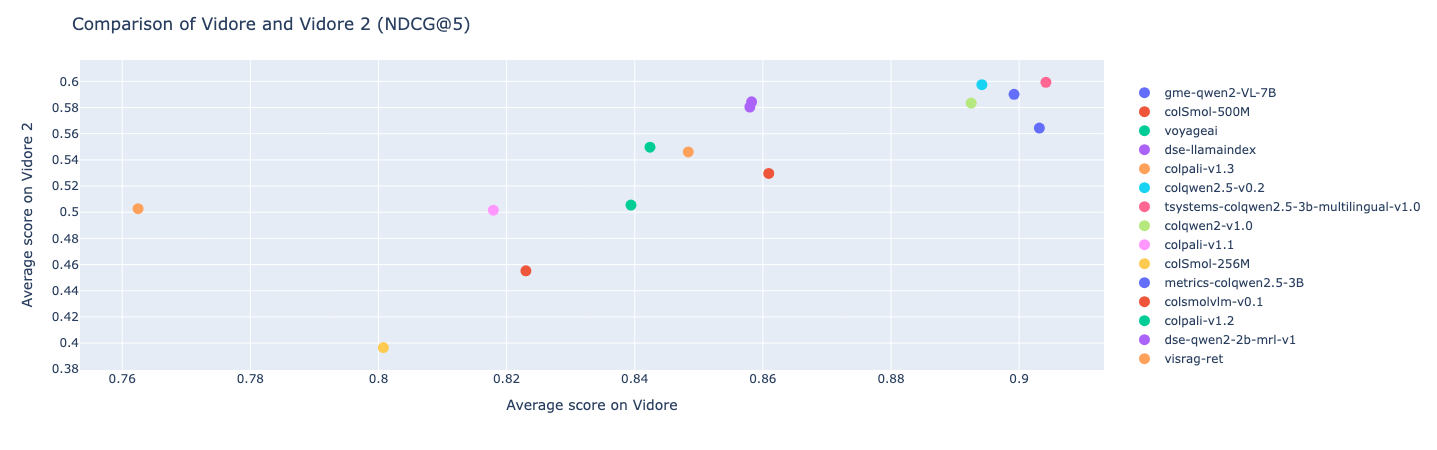
\includegraphics[width=\textwidth]{images/images_vidorev2/vsplot.png}
    \caption[V1 vs V2 performance]{V1 vs V2 performance comparison. V2 preserves model ranking signal while avoiding V1 saturation at the top end.}
    \label{fig:vidore-v1-v2}
\end{figure*}

\paragraph{Takeaway from V2.}
ViDoRe V2 successfully reintroduced discriminative power for retrieval evaluation, especially on cross-lingual and harder multi-page settings. It established the methodological foundations used in V3, but still remained primarily retrieval-centered.

\section{ViDoRe V3: benchmarking end-to-end multimodal RAG}

Building on V2, ViDoRe V3 broadens the scope from retrieval-only evaluation to full multimodal RAG assessment, including retrieval, answer generation, and visual grounding.

\begin{figure*}[h]
    \centering
    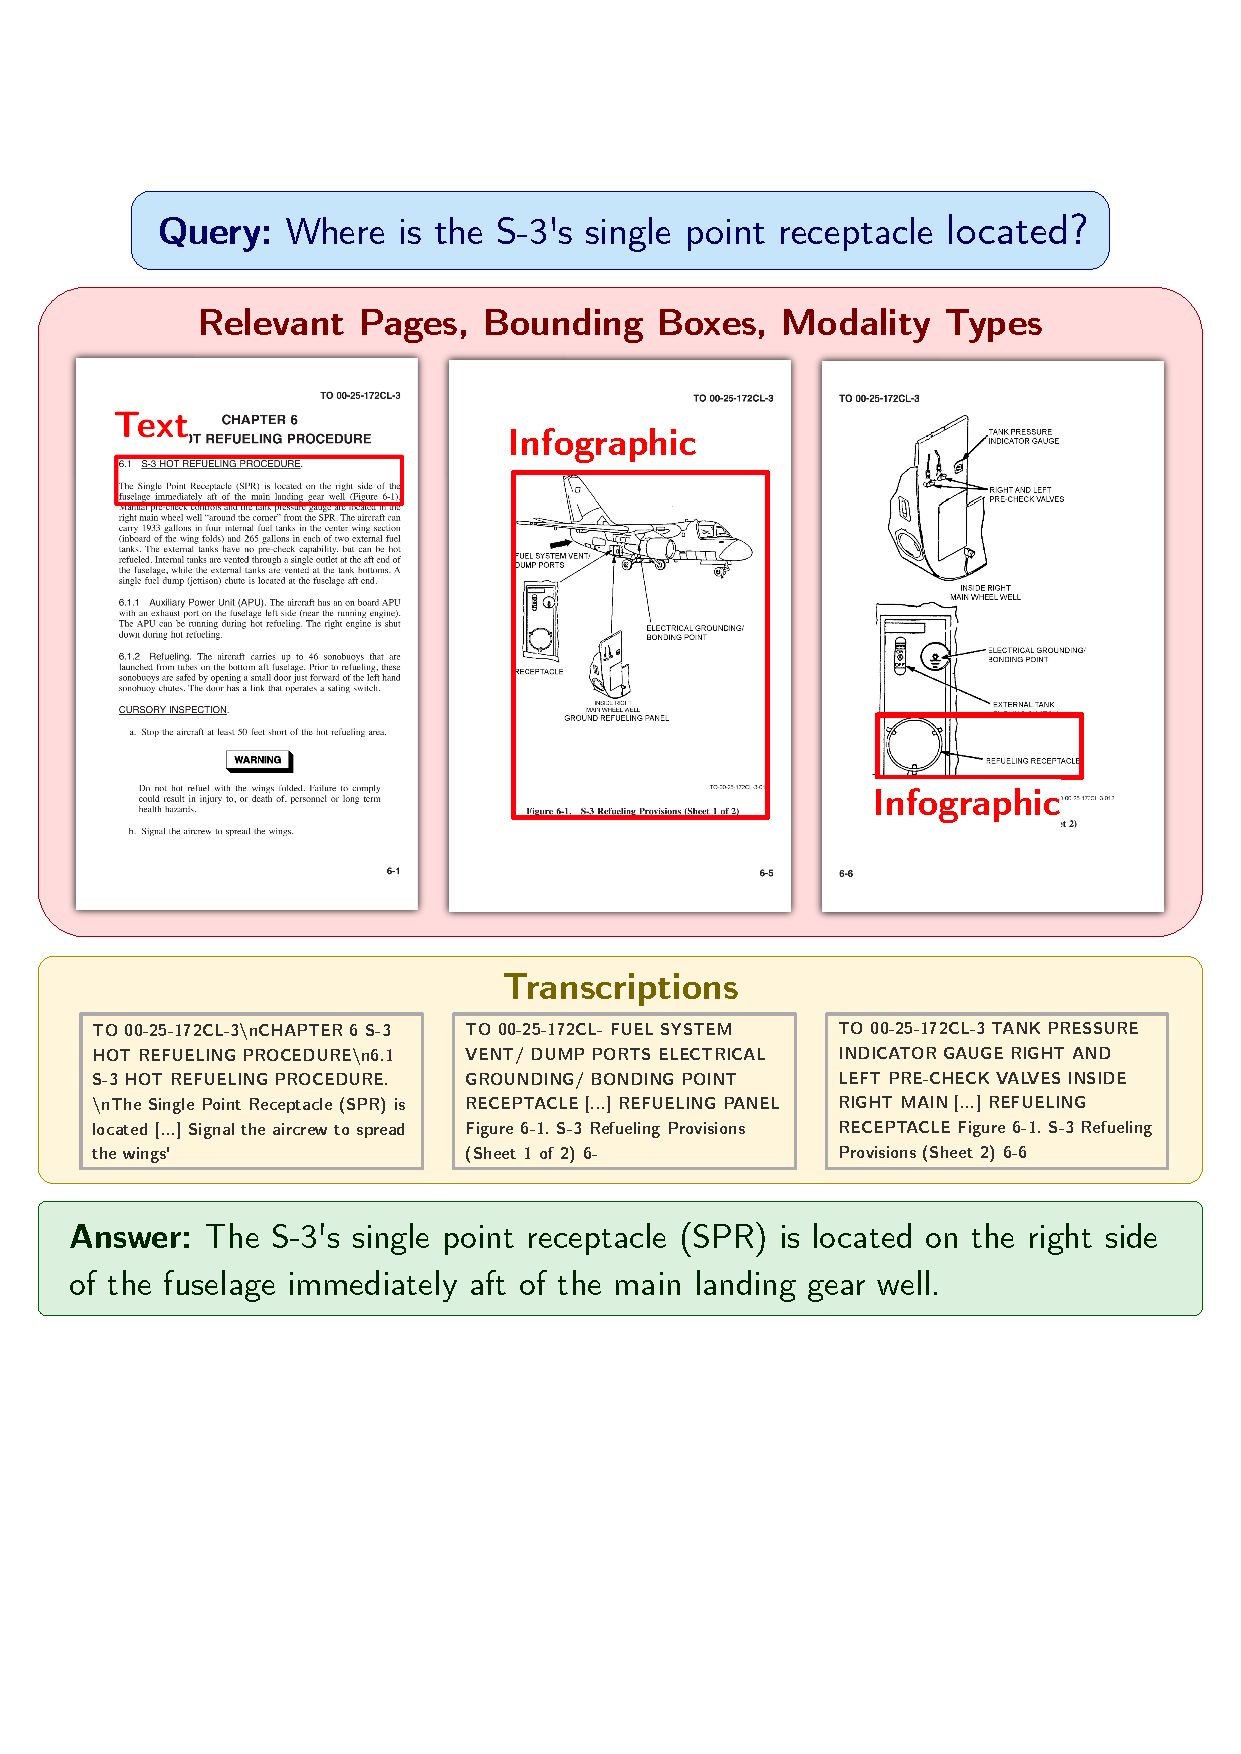
\includegraphics[trim={2cm 6.5cm 2cm 3.5cm}, clip, width=0.9\textwidth]{images/vidorev3_images/vidore_sample.pdf}
    \caption[ViDoRe V3 annotated sample]{\textbf{ViDoRe V3 annotated sample.} Each query is paired with relevant pages, a grounded reference answer, and supporting evidence boxes with modality labels.}
    \label{fig:vidorev3-sample}
\end{figure*}

\subsection{Why V3 was needed}

Practical RAG pipelines face difficulties that are underrepresented in many existing benchmarks:\
(1) information is often carried by visual structures (tables, charts, figures),\
(2) queries are frequently open-ended and require synthesis across documents, and\
(3) trustworthy answers need traceable grounding in source regions \sidecite{cho2024m3docragmultimodalretrievalneed, peng2025unidocbenchunifiedbenchmarkdocumentcentric, thakur2025freshstackbuildingrealisticbenchmarks}.

V3 was designed to evaluate these dimensions jointly and systematically.

\subsection{Scale and annotation workflow}

ViDoRe V3 covers 10 professional-domain datasets, around 26,000 pages, and 3,099 human-verified queries translated to 6 languages. The benchmark was built with a large human-in-the-loop pipeline (about 12,000 annotation hours), coupling VLM pre-filtering with expert review.

\begin{figure*}[t!]
    \centering
    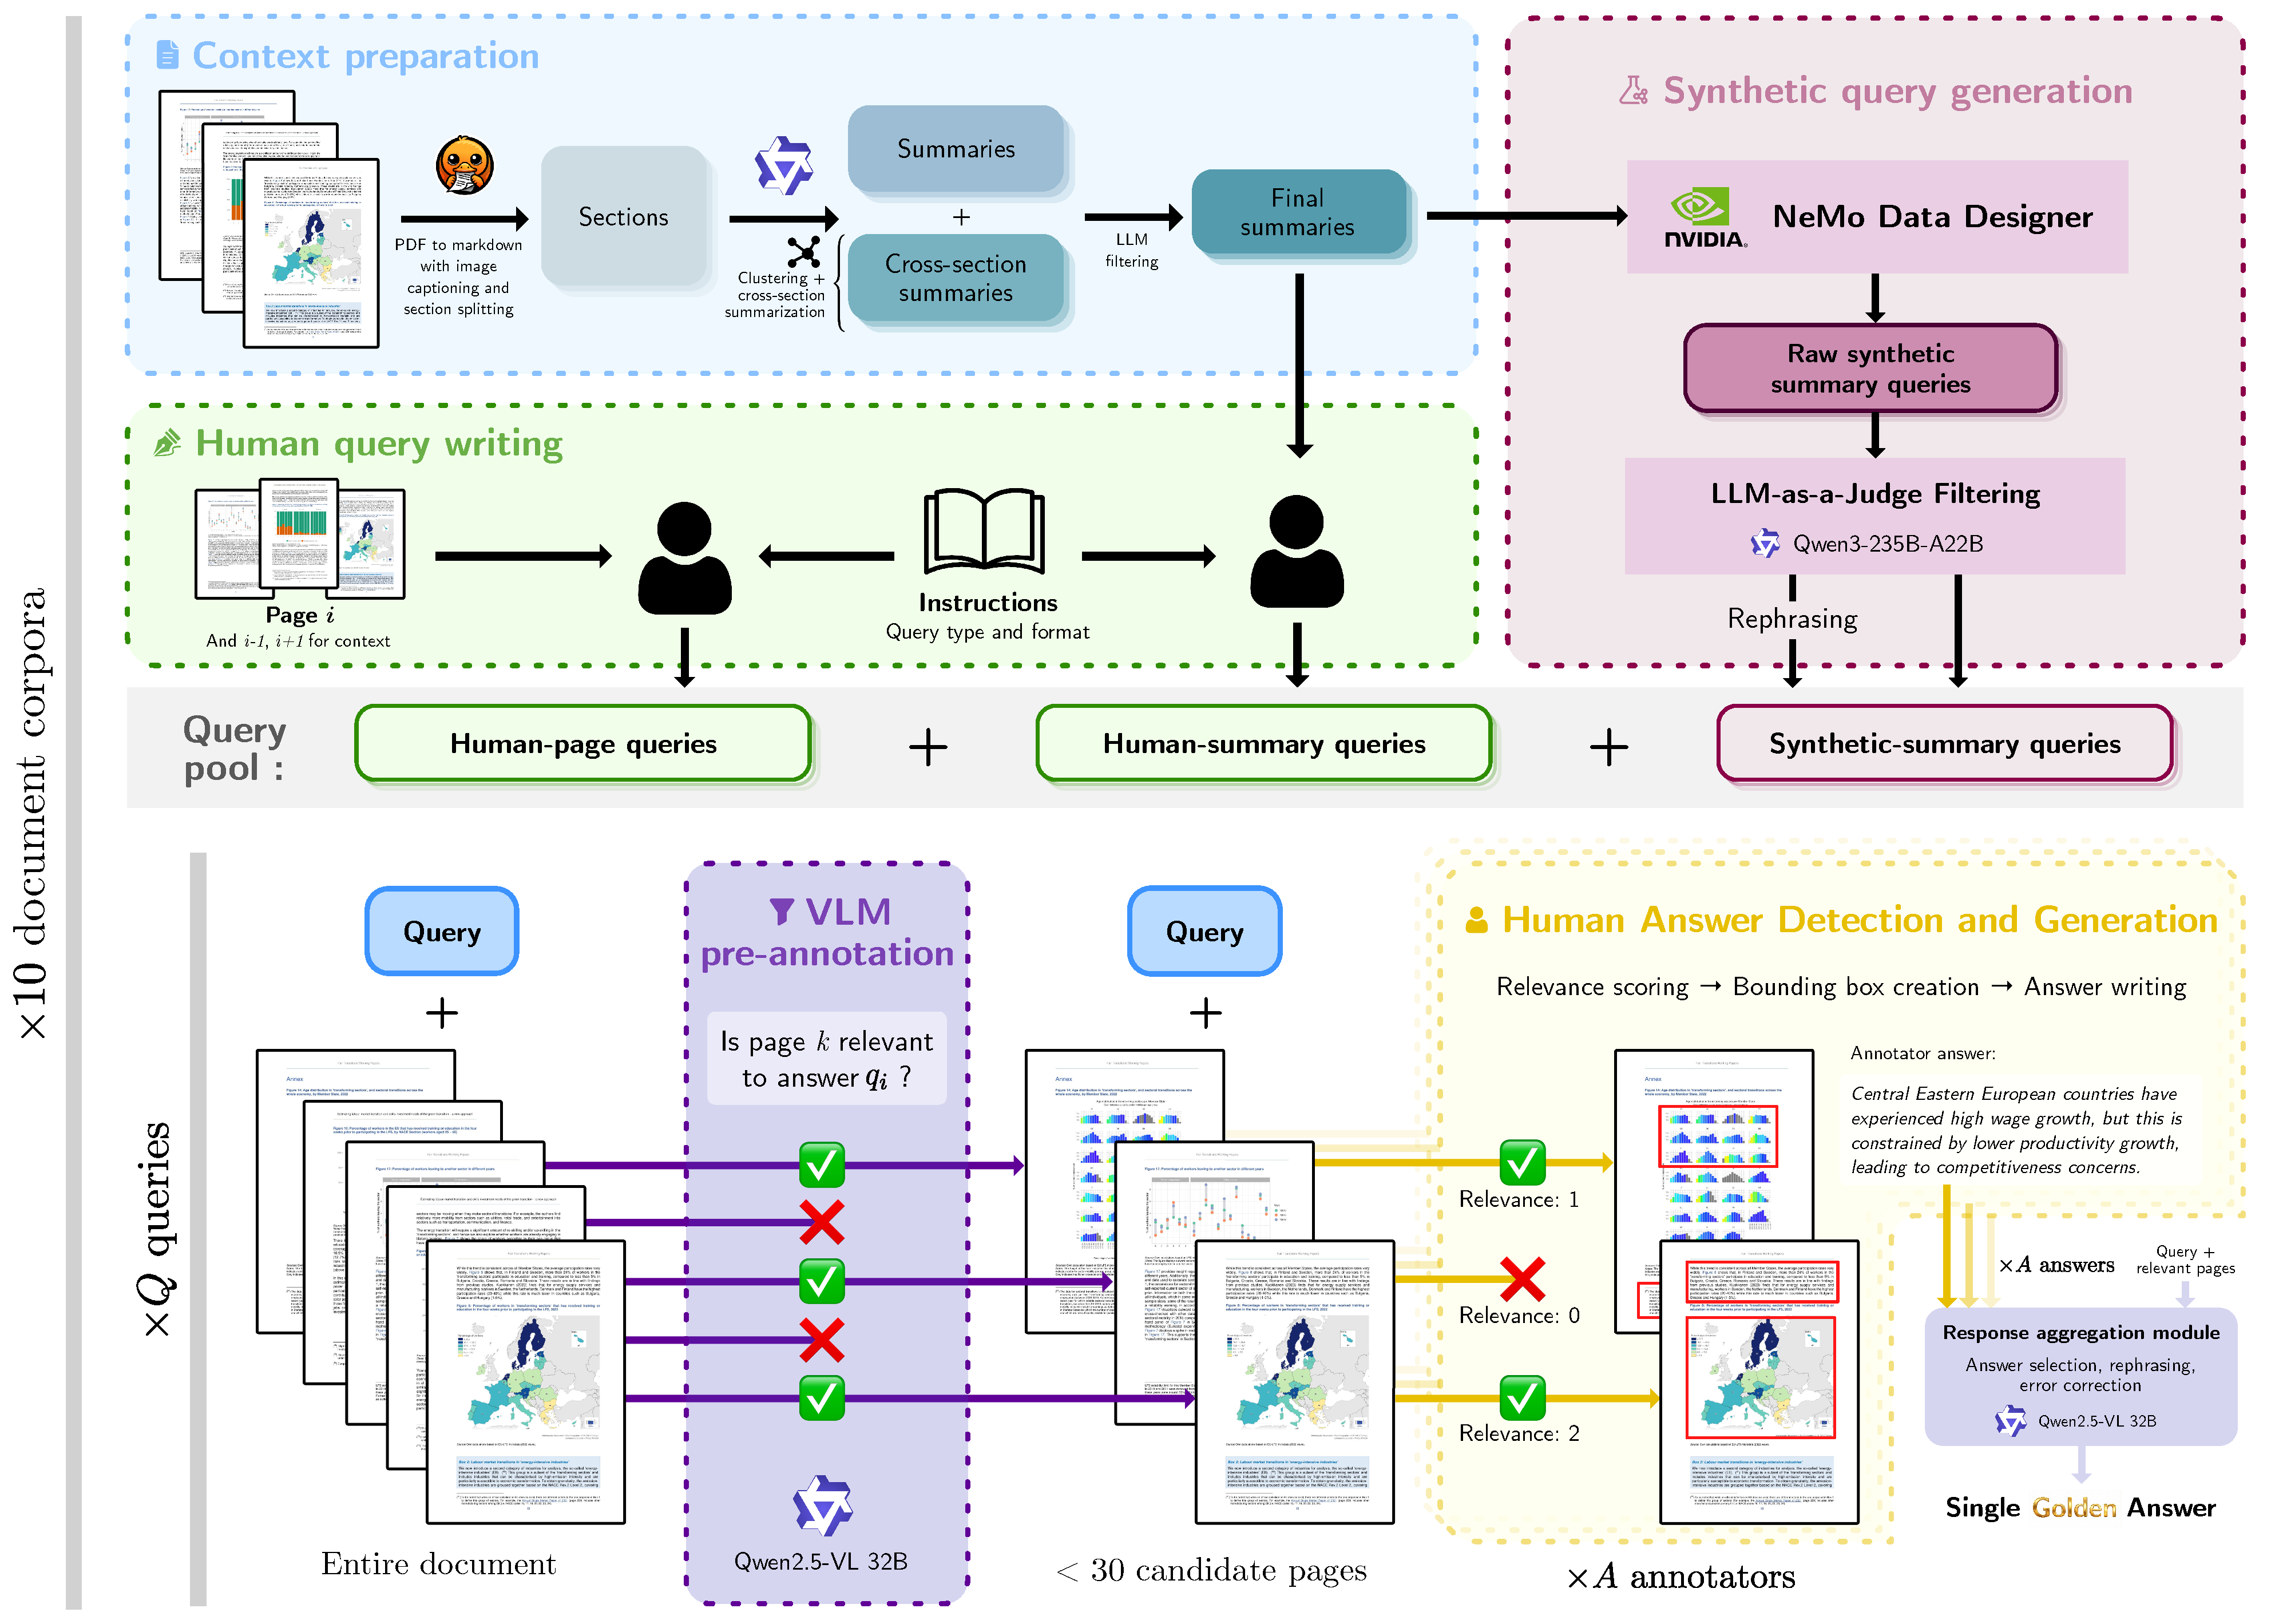
\includegraphics[width=1.25\textwidth]{images/vidorev3_images/dataset-generation-vf.pdf}
    \caption[ViDoRe V3 creation workflow]{\textbf{ViDoRe V3 data creation workflow.} Queries come from human extractive, human blind contextual, and synthetic blind contextual streams, followed by relevance annotation, answer writing, and evidence localization.}
    \label{fig:vidorev3-workflow}
\end{figure*}

\paragraph{Key annotation outputs.}
For each query-page pair, V3 stores (i) relevance labels, (ii) answer supervision, and (iii) grounding annotations via bounding boxes and modality tags. This makes it possible to diagnose where a pipeline fails: retrieval, reasoning, or localization.

\subsection{Query and content distributions}

A benchmark designed for realistic RAG should cover both diverse user intent and varied evidence modality. V3 includes query-type diversity (extractive, open-ended, boolean, numerical, multi-hop, etc.) and non-text evidence beyond pure OCR text.

\begin{figure}[ht]
    \centering
    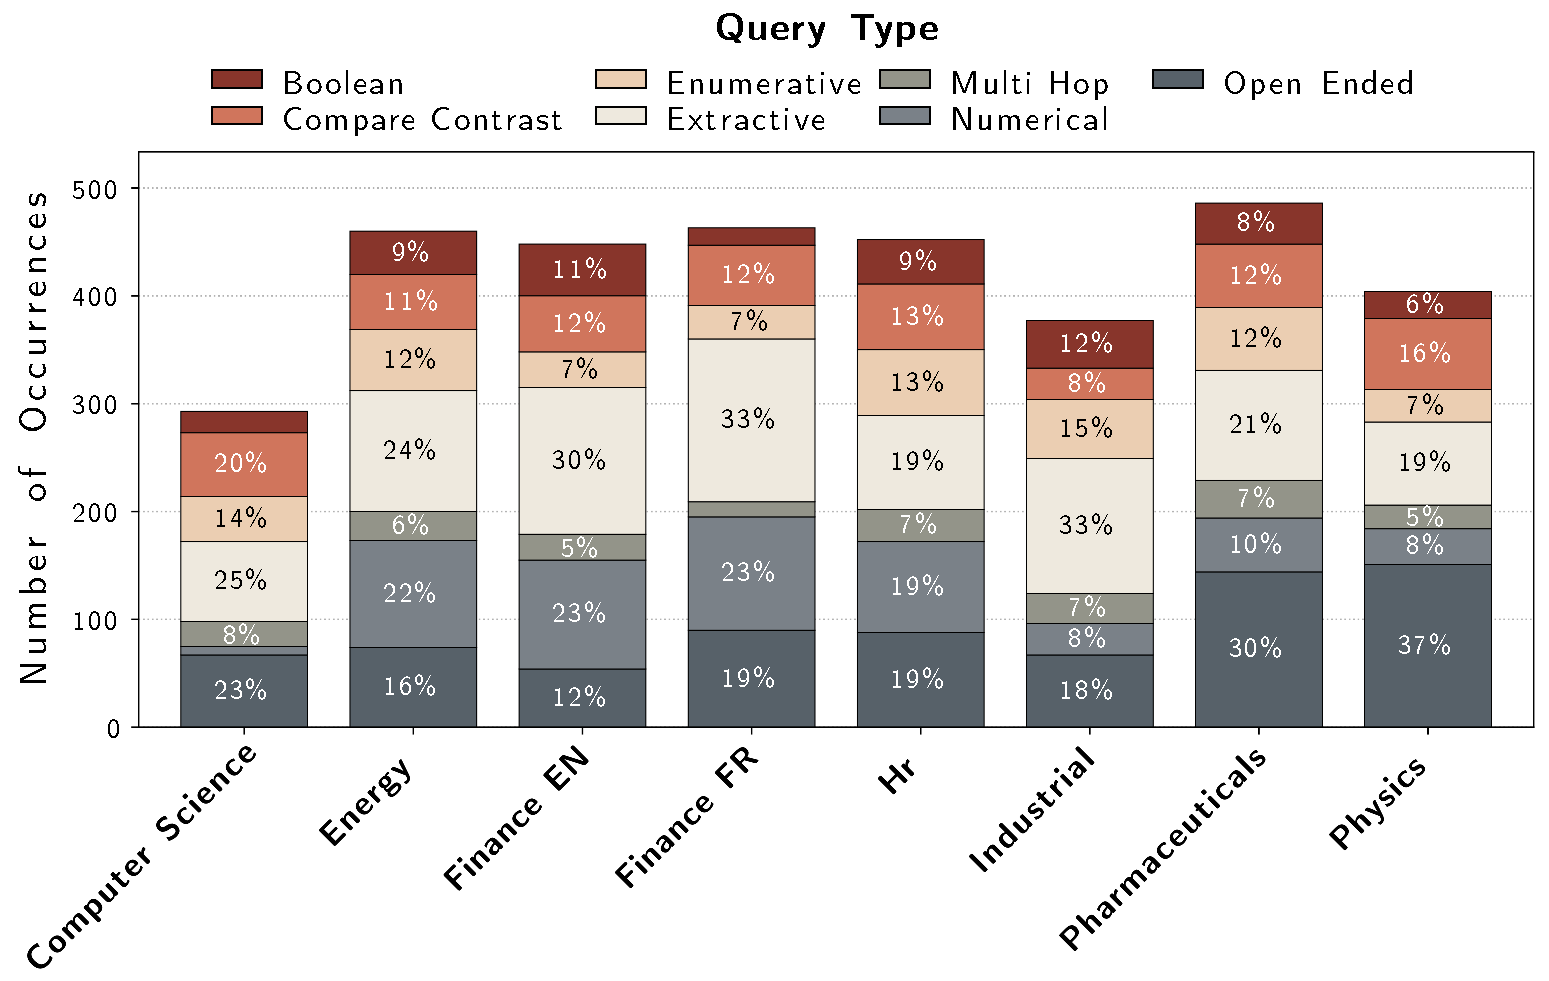
\includegraphics[width=0.9\textwidth]{images/vidorev3_images/vidore_distribution_acl_v2.pdf}
    \caption[Query type distribution by domain]{\textbf{Query type distribution by domain.} Relative frequencies across benchmark domains.}
    \label{fig:vidorev3-query-distribution}
\end{figure}

\begin{figure}[ht]
    \centering
    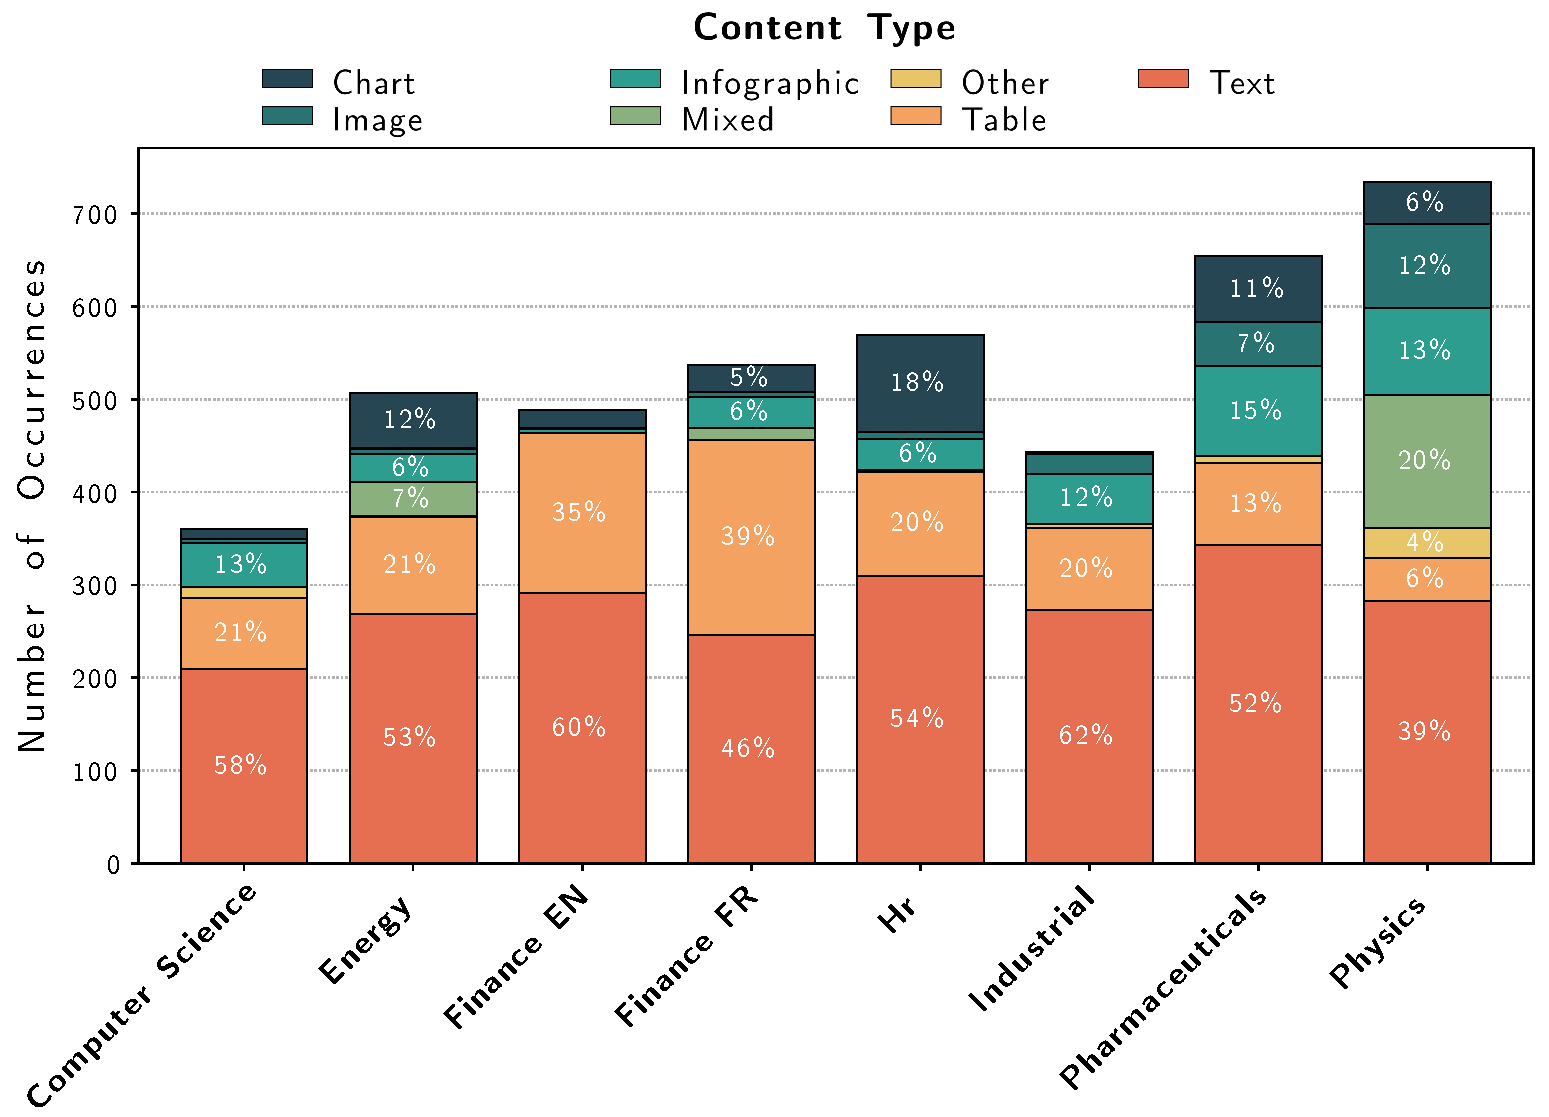
\includegraphics[width=0.9\textwidth]{images/vidorev3_images/content_type_distribution_acl_v2.pdf}
    \caption[Content type distribution by domain]{\textbf{Content type distribution by domain.} Relative frequencies of evidence modalities across domains.}
    \label{fig:vidorev3-content-distribution}
\end{figure}

\section{V3 retrieval results and analysis}

\subsection{Textual vs visual retrievers}

We evaluate strong textual and visual retrieval systems with NDCG@10. Results below show that visual late-interaction retrievers outperform textual baselines at comparable scale on this benchmark.

\begin{table*}[h!]
\small
\centering
\resizebox{1.18\textwidth}{!}{%
\begin{tabular}{l c c c c c c c c c c c >{\columncolor{avgcol}}c}
\toprule
 & & \multicolumn{7}{c}{\textbf{English Datasets}} & \multicolumn{3}{c}{\textbf{French Datasets}} & \multicolumn{1}{c}{} \\
\cmidrule(lr){3-9} \cmidrule(lr){10-12}
\textbf{Model} & Size (B) & \shortstack{C.S.} & \shortstack{Nucl.} & \shortstack{Fin.} & \shortstack{Phar.} & \shortstack{H.R.} & \shortstack{Ind.} & \shortstack{Tel.} & \shortstack{Phys.} & \shortstack{Ener.} & \shortstack{Fin.} & \textbf{Avg.} \\
\midrule
\multicolumn{13}{l}{\textit{\textbf{Textual Retrievers}}} \\
Qwen3-8B$^\bigstar$  & 8 & \textbf{71.7} & 39.0 & \textbf{49.4} & \textbf{59.2} & 47.6 & \textbf{40.4} & \textbf{62.8} & \textbf{45.6} & 58.9 & 35.8 & \textbf{51.0} \\
Jina-v4 & 3 & 64.3 & \textbf{44.3} & 48.4 & 54.9 & \textbf{52.8} & 38.4 & 56.3 & 43.6 & \textbf{60.1} & \textbf{41.3} & 50.4 \\
LFM2-350M & 0.35 & 63.5 & 37.8 & 39.0 & 56.4 & 43.5 & 34.4 & 56.9 & 41.8 & 47.0 & 28.2 & 44.9 \\
Qwen3-0.6B$^\bigstar$  & 0.6 & 66.4 & 32.8 & 42.7 & 50.6 & 37.7 & 31.6 & 55.7 & 43.3 & 51.3 & 25.8 & 43.8 \\
BGE-M3$^\bigstar$  & 0.57 & 58.0 & 30.2 & 39.8 & 52.0 & 42.4 & 28.5 & 51.6 & 35.9 & 49.8 & 25.2 & 41.3 \\
BM25S & - & 28.7 & 17.4 & 17.6 & 27.3 & 12.8 & 15.6 & 33.3 & 14.8 & 21.9 & 14.0 & 20.3 \\
\midrule
\multicolumn{13}{l}{\textit{\textbf{Visual Retrievers}}} \\
ColEmbed-3B-v2 & 3 & \textbf{77.1} & \textbf{50.7} & \textbf{64.2 }& \textbf{66.0} & \textbf{62.3} & \textbf{51.7} & \textbf{69.7} & 47.0 & 64.9 & 44.4 & \textbf{59.8} \\
Jina-v4 & 3 & 71.8 & 50.0 & 59.3 & 63.1 & 59.5 & 50.4 & 64.8 & 46.6 & 64.0 & \textbf{46.1} & 57.6 \\
ColNomic-7B & 7 & 76.2 & 45.0 & 56.6 & 62.3 & 58.7 & 50.1 & 67.2 & \textbf{48.3} & 64.0 & 45.5 & 57.4 \\
ColEmbed-3B & 3 & 75.2 & 49.1 & 60.9 & 63.7 & 58.7 & 47.1 & 67.0 & 45.1 & 62.1 & 43.8 & 57.3 \\
ColNomic-3B & 3 & 72.7 & 42.1 & 56.3 & 61.1 & 57.3 & 47.4 & 64.5 & 47.5 & \textbf{65.0} & 44.3 & 55.8 \\
ColEmbed-1B & 1 & 71.3 & 47.3 & 58.9 & 62.6 & 57.0 & 46.6 & 64.7 & 44.1 & 60.9 & 42.4 & 55.6 \\
ColQwen2.5 & 3 & 72.3 & 38.1 & 52.3 & 57.9 & 51.2 & 41.3 & 61.3 & 45.9 & 59.7 & 39.1 & 51.9 \\
Nomic-7B$^\bigstar$  & 7 & 66.6 & 36.7 & 48.8 & 58.9 & 46.2 & 37.9 & 57.8 & 44.2 & 57.5 & 36.0 & 49.0 \\
ColQwen2 & 2 & 68.6 & 35.7 & 39.0 & 52.2 & 45.1 & 38.3 & 57.4 & 41.6 & 48.8 & 20.0 & 44.7 \\
Nomic-3B$^\bigstar$ & 3 & 58.5 & 32.2 & 44.2 & 55.3 & 43.3 & 33.2 & 53.7 & 42.0 & 51.4 & 28.9 & 44.3 \\
ColPali & 7 & 65.3 & 32.9 & 34.4 & 53.1 & 44.8 & 35.6 & 54.0 & 41.7 & 47.1 & 21.8 & 43.1 \\
\bottomrule
\end{tabular}
}
\caption[Retriever performance across ViDoRe V3]{\textbf{Retrieval performance (NDCG@10) across ViDoRe V3.} Best values within each category are bolded.}
\label{tab:vidorev3-retriever-comparison}
\end{table*}

\paragraph{Main retrieval observations.}
Three trends stand out: (i) visual retrievers are consistently stronger than textual retrievers on visually rich pages; (ii) late-interaction models lead dense single-vector variants; and (iii) performance decreases for harder query classes requiring multi-step synthesis.

\begin{figure}[ht]
    \centering
    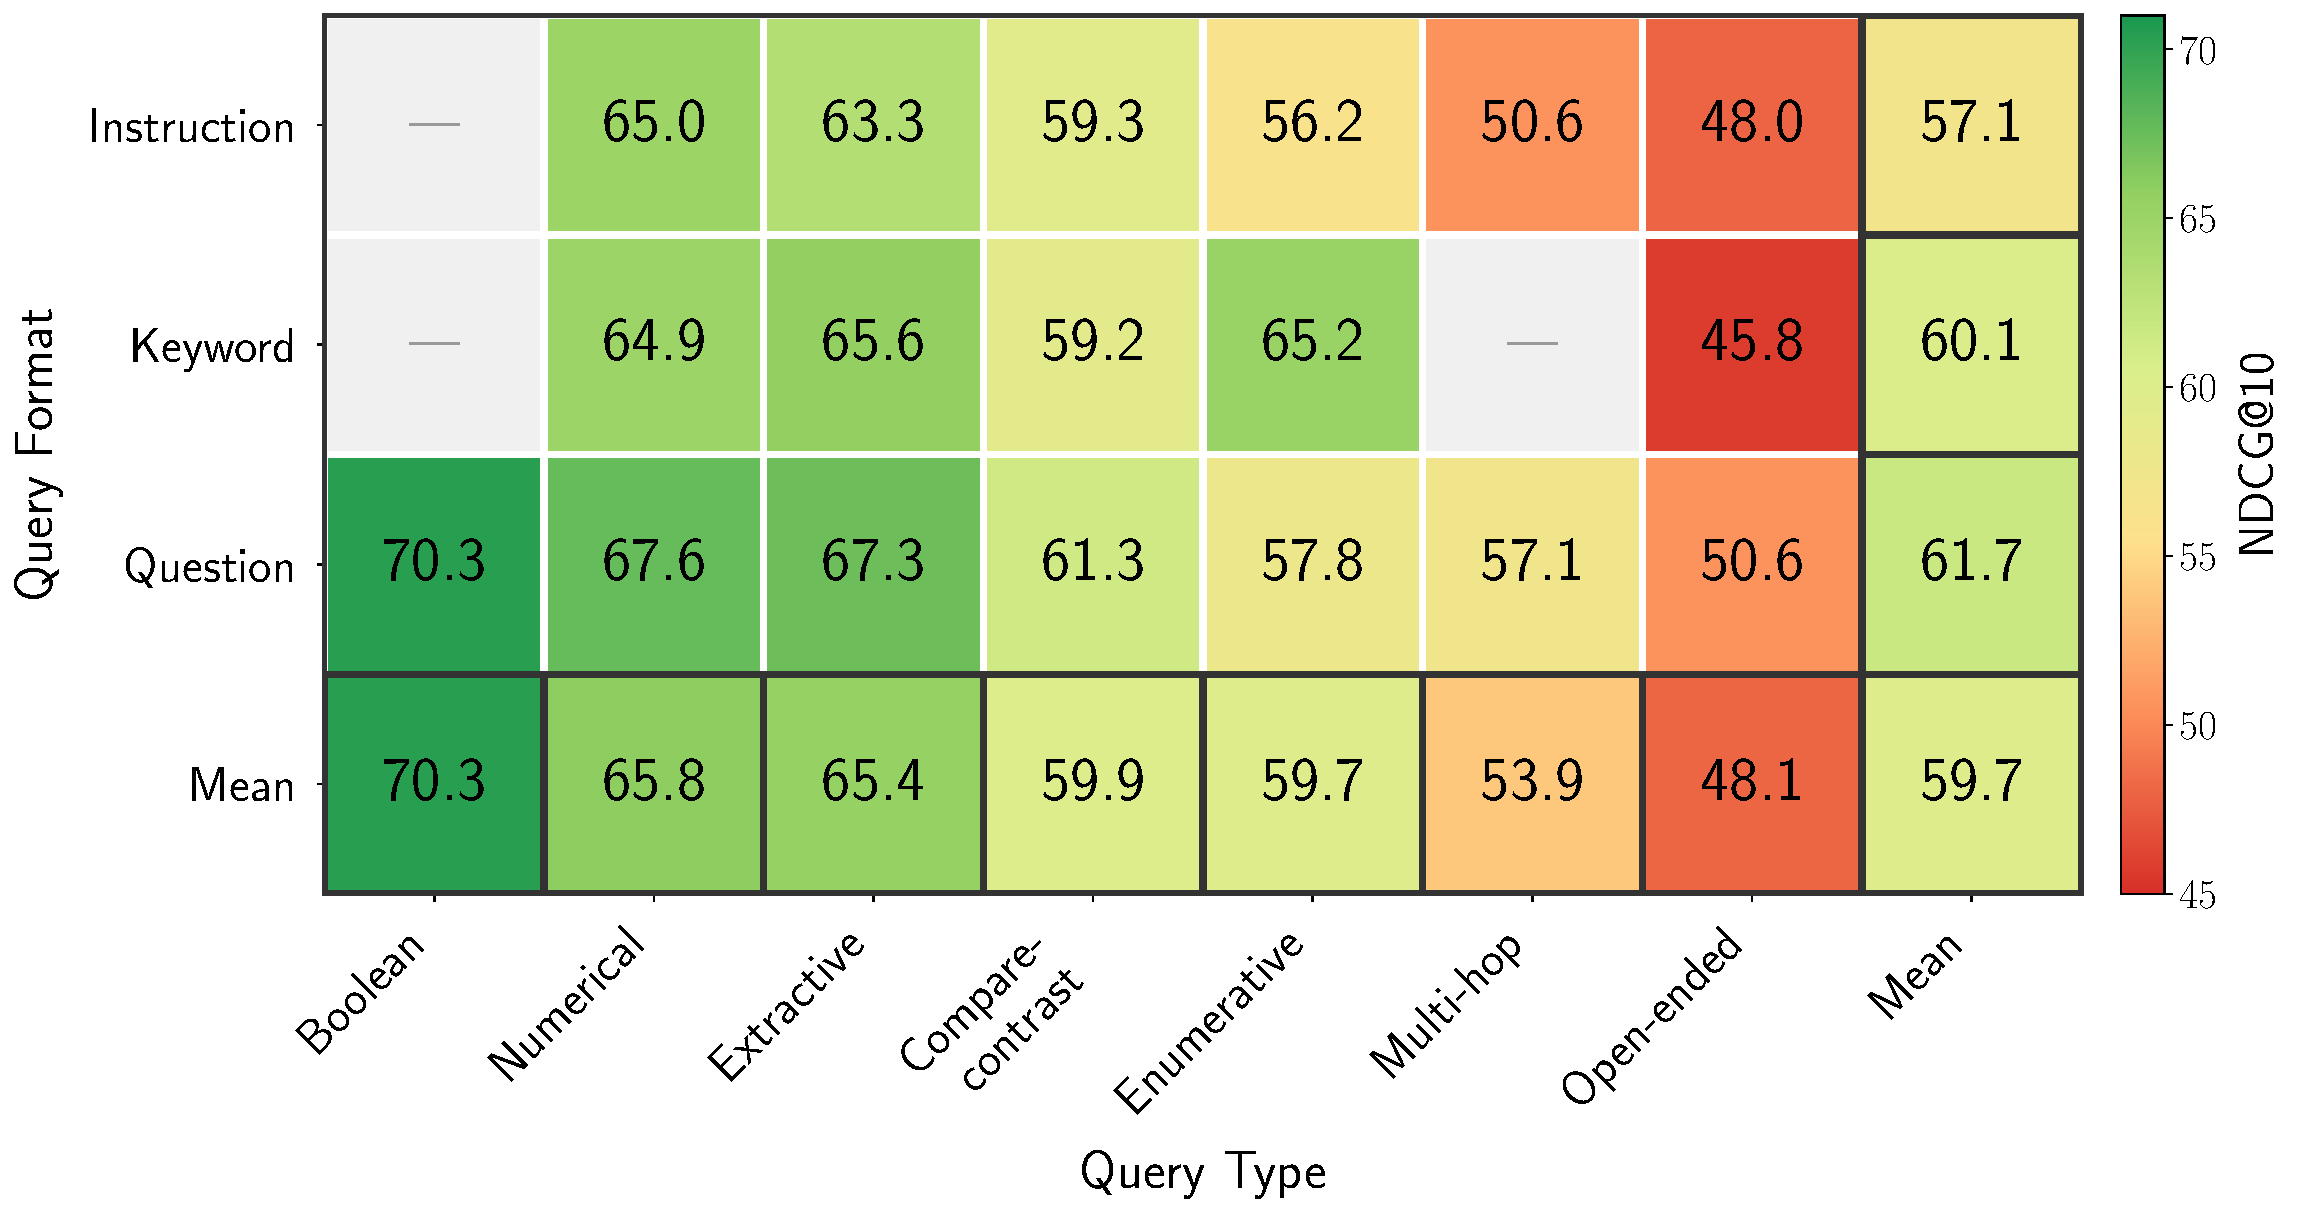
\includegraphics[width=0.98\textwidth]{images/vidorev3_images/ndcg_by_type_format_transposed.pdf}
    \caption[Performance by query type and format]{\textbf{ColEmbed-3B-v2 by query type and format (NDCG@10).} Simpler query types are easier; open-ended and multi-hop formulations remain challenging.}
    \label{fig:vidorev3-type-format}
\end{figure}

\begin{figure}[ht]
    \centering
    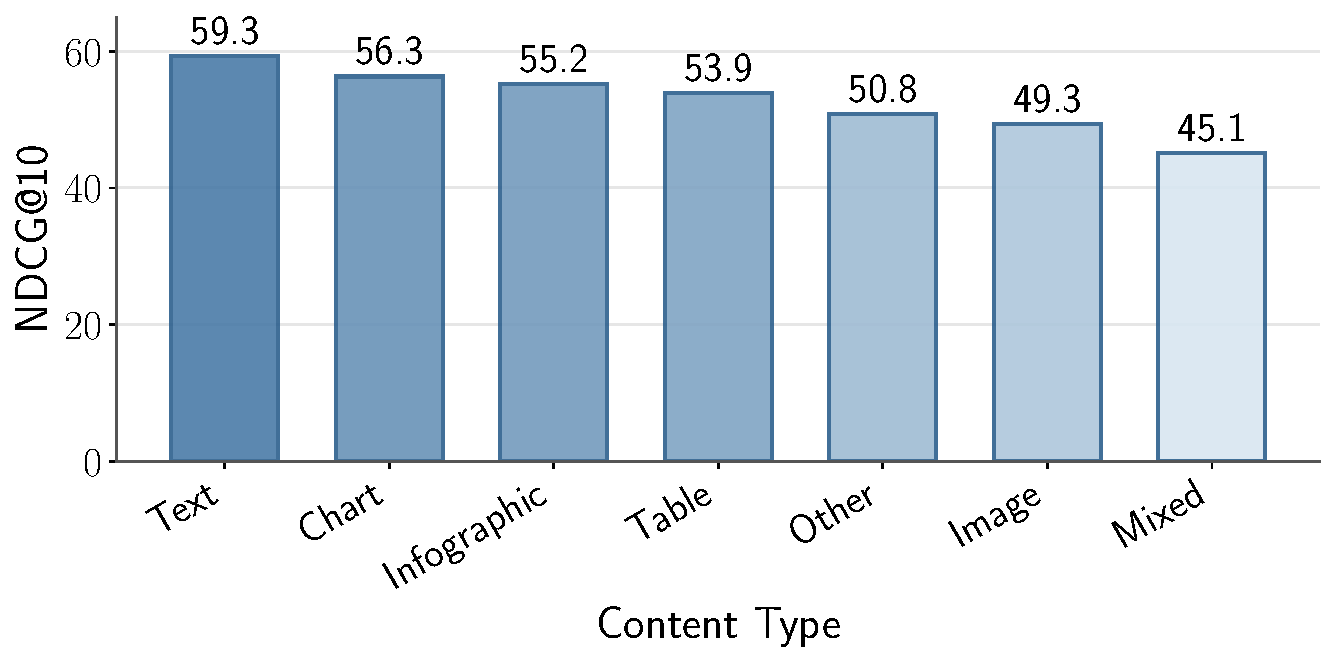
\includegraphics[width=0.65\textwidth]{images/vidorev3_images/ndcg_by_content_type.pdf}
    \caption[Performance by evidence modality]{\textbf{ColEmbed-3B-v2 by evidence modality (NDCG@10).} Mixed and visual-heavy evidence remains comparatively difficult.}
    \label{fig:vidorev3-content-type}
\end{figure}

\begin{figure}[ht]
    \centering
    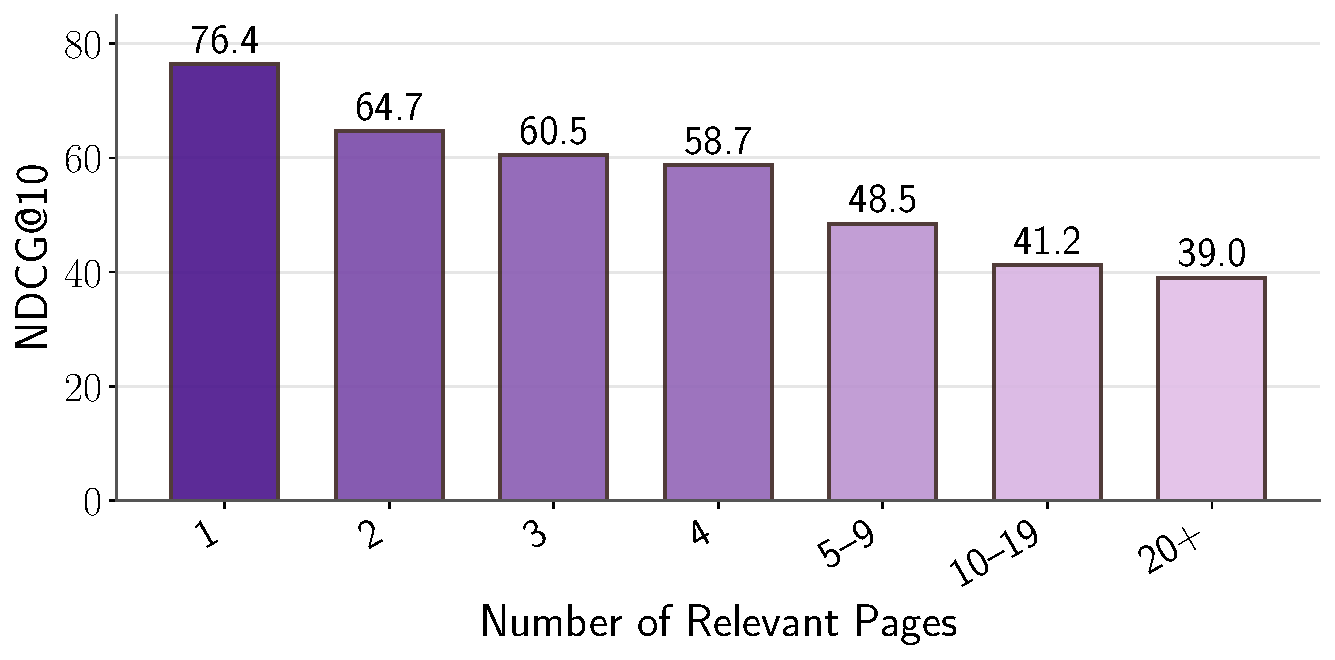
\includegraphics[width=0.65\textwidth]{images/vidorev3_images/ndcg_by_relevant_pages.pdf}
    \caption[Performance by number of relevant pages]{\textbf{ColEmbed-3B-v2 by number of relevant pages (NDCG@10).} As answers spread over more pages, retrieval quality drops.}
    \label{fig:vidorev3-num-pages}
\end{figure}

\subsection{Reranking analysis}

We compare strong textual and visual reranking setups on top of Jina-v4. Textual reranking yields large gains, while visual reranking currently provides only marginal improvements, suggesting reranker maturity is still modality-dependent.

\newcommand{\plus}[1]{\textcolor{teal}{\tiny \textbf{$\uparrow$#1}}}
\newcommand{\minus}[1]{\textcolor{red}{\tiny \textbf{$\downarrow$#1}}}
\newcommand{\val}[2]{\shortstack{#1 \\[-0.2em] \hspace{1.3em}#2}}
\begin{table*}[h]
    \centering
    \small
    \setlength{\tabcolsep}{3pt}
    \resizebox{1.18\textwidth}{!}{%
    \begin{tabular}{l ccccccc ccc >{\columncolor{avgcol}}c}
        \toprule
         & \multicolumn{7}{c}{\textbf{English Datasets}} & \multicolumn{3}{c}{\textbf{French Datasets}} & \multicolumn{1}{c}{} \\
        \cmidrule(lr){2-8} \cmidrule(lr){9-11}
        \textbf{Model}& \shortstack{C.S.} & \shortstack{Nucl.} & \shortstack{Fin.} & \shortstack{Phar.} & \shortstack{H.R.} & \shortstack{Ind.} & \shortstack{Tel.} & \shortstack{Phys.} & \shortstack{Ener.} & \shortstack{Fin.} & \textbf{Avg.} \\
        \midrule
        \textit{\textbf{Textual pipeline}} & \multicolumn{11}{c}{}\\
        \multirow[c]{2}{*}{\makecell[l]{Jina-v4\textsuperscript{textual} \\+ zerank-2}} &
        64.3 & 44.3 & 48.4 & 54.9 & 52.8 & 38.4 & 56.3 & 43.6 & 60.1 & 41.3 & 50.4 \\
         &
        \val{\textbf{82.1}}{\plus{17.8}} &
        \val{\textbf{53.5}}{\plus{9.2}} &
        \val{\textbf{69.2}}{\plus{20.8}} &
        \val{\textbf{66.2}}{\plus{11.3}} &
        \val{\textbf{66.5}}{\plus{13.7}} &
        \val{\textbf{53.2}}{\plus{14.8}} &
        \val{\textbf{71.5}}{\plus{15.2}} &
        \val{\textbf{48.2}}{\plus{4.6}} &
        \val{\textbf{71.5}}{\plus{11.4}} &
        \val{\textbf{53.7}}{\plus{12.4}} &
        \val{\textbf{63.6}}{\plus{13.2}}
        \\
        \midrule
        \textit{\textbf{Visual pipeline}} & \multicolumn{11}{c}{} \\
        \multirow[c]{2}{*}{\makecell[l]{Jina-v4\textsuperscript{visual} \\+ jina-reranker-m0}} & 71.8 & 50.0 & 59.3 & 63.1 & 59.5 & 50.4 & 64.8 & 46.6 & 64.0 & 46.1 & 57.6 \\
        &
        \val{76.7}{\plus{4.9}} &
        \val{50.8}{\plus{0.8}} &
        \val{59.2}{\minus{0.1}} &
        \val{65.4}{\plus{2.3}} &
        \val{56.0}{\minus{3.5}} &
        \val{50.9}{\plus{0.5}} &
        \val{70.8}{\plus{6.0}} &
        \val{46.9}{\plus{0.3}} &
        \val{61.7}{\minus{2.3}} &
        \val{39.8}{\minus{6.3}} &
        \val{57.8}{\plus{0.2}} \\
        \bottomrule
    \end{tabular}
    }
    \caption[Reranking pipeline performance]{\textbf{Retriever + reranker performance (NDCG@10).} Textual reranking yields large gains; visual reranking gains are limited and unstable across datasets.}
    \label{tab:vidorev3-reranking}
\end{table*}

\section{End-to-end answer generation in V3}

Beyond retrieval, we evaluate final answer correctness across retrieval pipelines, context modalities (text/image/hybrid), and generation models. We also report oracle-context upper bounds.

\begin{table*}[h!]
\centering
\small
\resizebox{\textwidth}{!}{%
\begin{tabular}{l l l ccccc ccc >{\columncolor{avgcol}}c c c}
\toprule
& & & \multicolumn{5}{c}{\textbf{English Datasets}} & \multicolumn{3}{c}{\textbf{French Datasets}} & \cellcolor{white}& & \cellcolor{white} \\
\cmidrule(lr){4-8} \cmidrule(lr){9-11}
\makecell[l]{\textbf{Retrieval} \\ \textbf{pipeline}} & \makecell[l]{\textbf{Context} \\ \textbf{modality}} & \makecell[l]{\textbf{Generation} \\ \textbf{model}} & \makecell{C.S.} & \makecell{Fin.} & \makecell{Phar.} & \makecell{H.R.} & \makecell{Ind.} & \makecell{Phys.} & \makecell{Ener.} & \makecell{Fin.} & \makecell{\textbf{Avg.}\\\textbf{Hard}}& \makecell{Avg.\\Easy} & \makecell{Avg.\\Global} \\
\midrule
\multirow{3}{*}{Oracle} & Text & \multirow{3}{*}{Gemini 3 Pro} & 80.9 & 70.2 & 71.4 & \textbf{72.3} & 66.4 & 71.2 & 69.2 & 62.8 & 62.3& 79.3 & 70.6 \\
& Image & & \textbf{86.5} & \textbf{70.6} & \textbf{76.1} & 71.1 & \textbf{68.2} & 74.5 & \textbf{69.8} & \textbf{64.1} & \textbf{64.7}& \textbf{79.7} & \textbf{72.6} \\
& Hybrid & & 86.0 & 68.9 & 73.4 & 70.4 & 65.4 & 69.2 & 69.5 & 62.8 & 63.4& 77.5 & 70.7 \\
\midrule
\makecell[l]{Jina-v4\textsuperscript{text.} + zerank-2} & Text & Gemini 3 Pro & 80.9 & 66.0 & 59.9 & 63.2 & 60.4 & 69.2 & 64.9 & \underline{54.7} & 52.1& 75.5 & 64.9 \\
\midrule
\makecell[l]{Jina-v4\textsuperscript{text.} + zerank-2 \\ \& ColEmbed-3B-v2} & Hybrid & Gemini 3 Pro & 85.1 & 65.0 & 65.9 & 64.8 & 59.4 & 69.9 & 62.7 & 52.8 & \underline{54.7}& 76.6 & 65.7 \\
\midrule
\multirow{6}{*}{ColEmbed-3B-v2} & \multirow{2}{*}{Text} & Gemini 3 Pro & 82.3 & 62.5 & 61.0 & 62.9 & 56.2 & 64.9 & 62.3 & 49.4 & 51.7& 73.0 & 62.7 \\
 & & Kimi K2 & 81.4 & 56.6 & 59.1 & 55.7 & 55.8 & 73.8 & 60.4 & 43.1 & 44.6& 74.3 & 60.7 \\
\cmidrule{2-14}
& \multirow{4}{*}{Image} & Gemini 3 Pro & 83.3 & \underline{67.3} & 62.9 & 65.4 & 57.2 & 67.9 & 64.3 & 47.8 & 54.5& 74.1 & 64.5 \\
 & & Gemini 3 Flash & 80.9 & 64.1 & 63.5 & 63.8 & 55.1 & 68.2 & 63.3 & 47.8 & 50.3& 74.4 & 63.3 \\
& & GPT-5.2 & \underline{\textbf{86.5}} & 59.5 & \underline{68.1} & \underline{66.0} & \underline{61.5} & \underline{\textbf{76.5}} & \underline{66.2} & 49.1 & 54.1& \underline{78.1} & \underline{66.7} \\
& & Qwen3-VL-235B & 86.0 & 59.9 & 64.0 & 60.7 & 57.2 & 71.9 & 59.7 & 44.4 & 51.0& 74.1 & 63.0 \\
\bottomrule
\end{tabular}
}
\caption[End-to-end answer accuracy]{\textbf{End-to-end answer accuracy.} Correct-answer rates across public datasets under different retrieval and generation setups.}
\label{tab:vidorev3-end-to-end}
\end{table*}

\paragraph{Generation insights.}
Three findings are particularly important for system design:
\begin{itemize}
    \item \textbf{Visual context is valuable}: image-based context often outperforms text-only context on harder queries.
    \item \textbf{Retrieval remains a bottleneck}: oracle rows are substantially above non-oracle pipelines, showing missed evidence still limits answer quality.
    \item \textbf{Hybrid strategies are competitive}: combining strong textual reranking with visual retrieval can improve robustness across datasets.
\end{itemize}

\section{Conclusion: what V3 changes in practice}

ViDoRe V2 was the critical transition benchmark that moved beyond V1 saturation through more realistic retrieval design. ViDoRe V3 extends this to a substantially richer benchmarking framework: multilingual, visually grounded, and end-to-end. It enables both leaderboard-style ranking and pipeline diagnostics, making it a practical tool for guiding the next generation of multimodal enterprise RAG systems.
